\documentclass[12pt,a4paper,fleqn]{article}
\title{Progress Report}
\author{Syed Ahmad Raza\\
        D10503816}
\date{2018.11.07}
\usepackage{mathtools}          % for math
\usepackage{graphicx}           % for graphics
\usepackage{booktabs}           % for professional tables
\usepackage{float}              % force a figure placement with [H] command
\usepackage{newtxtext}          % better text font
\usepackage{newtxmath}          % better math font
\usepackage{nicefrac}           % use nicer smaller fractions
\graphicspath{{../figures/}}    % only works when -shell-escape option is used with pdflatex
%\usepackage{enumitem}           % control layout of itemize and enumerate
%\usepackage{layouts}            % find \printinunitsof{in}\prntlen{\textwidth}
%\usepackage{xcolor}             % for using colors in document

\begin{document}
\maketitle
%\tableofcontents
%\pagebreak

\section{Testing parallelization of 3D code with OpenMP}

The three-dimensional solver for Navier-Stokes equations has been parallelized using OpenMP. Currently, only the pressure loop has been paralellized for validation and because the pressure loop is critical to the performance of the whole code due to its numerous iterations in time steps.

\section{Results and validation of three-dimensional solver}

The 3D solver was used to model a lid-driven cubic cavity flow for the case of \(\text{Re}=100\) with a \(41 \times 41 \times 41\) grid size. Simulation results from the parallelized code have been compared with the output from non-parallelized code and the published results of Ku et al. \cite{Ku:1987:PMS:33136.33145} for three-dimensional cubic cavity flow and Ghia et al. \cite{GHIA1982387} for two-dimensional square cavity flow. The figures below represent the comparison of \(x\)-direction velocity \(u\) on the vertical centerline and \(y\)-direction velocity \(v\) on the horizontal centerline of the cubic cavity at the mid-plane in \(z\)-direction.

\begin{figure}[H]
    \centering
    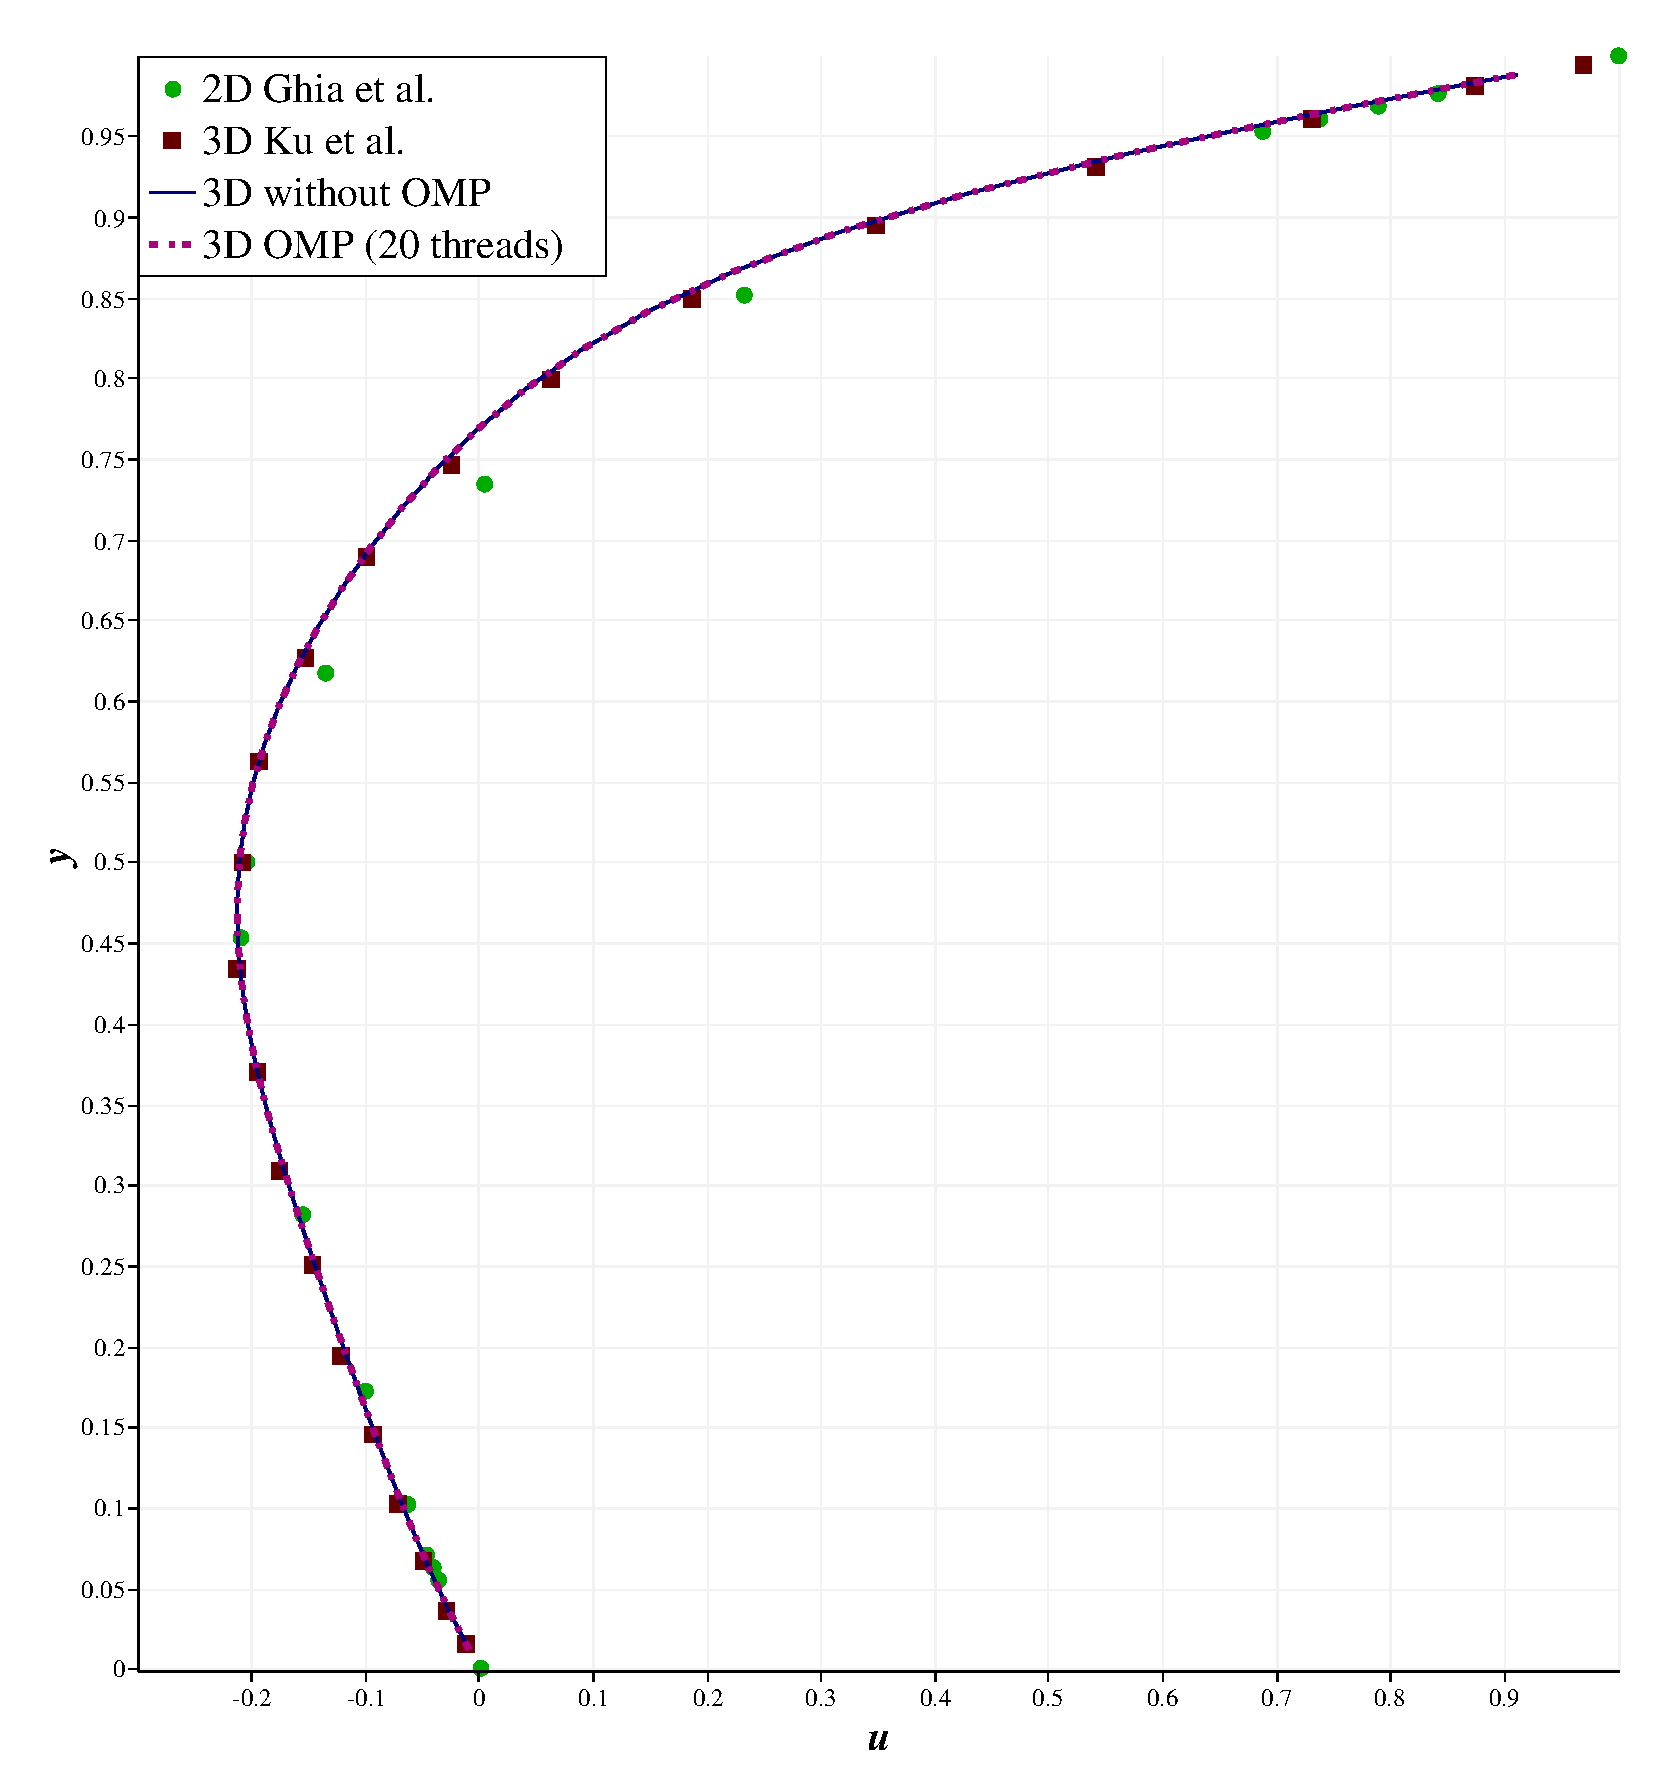
\includegraphics[width=\linewidth]{U-3D_ompValidation.eps}
    \caption{\(u\)-velocity profiles on the vertical centerline in cubic cavity (at the center of \(z\)-axis) for the various cases.}
\end{figure}

\begin{figure}[H]
    \centering
    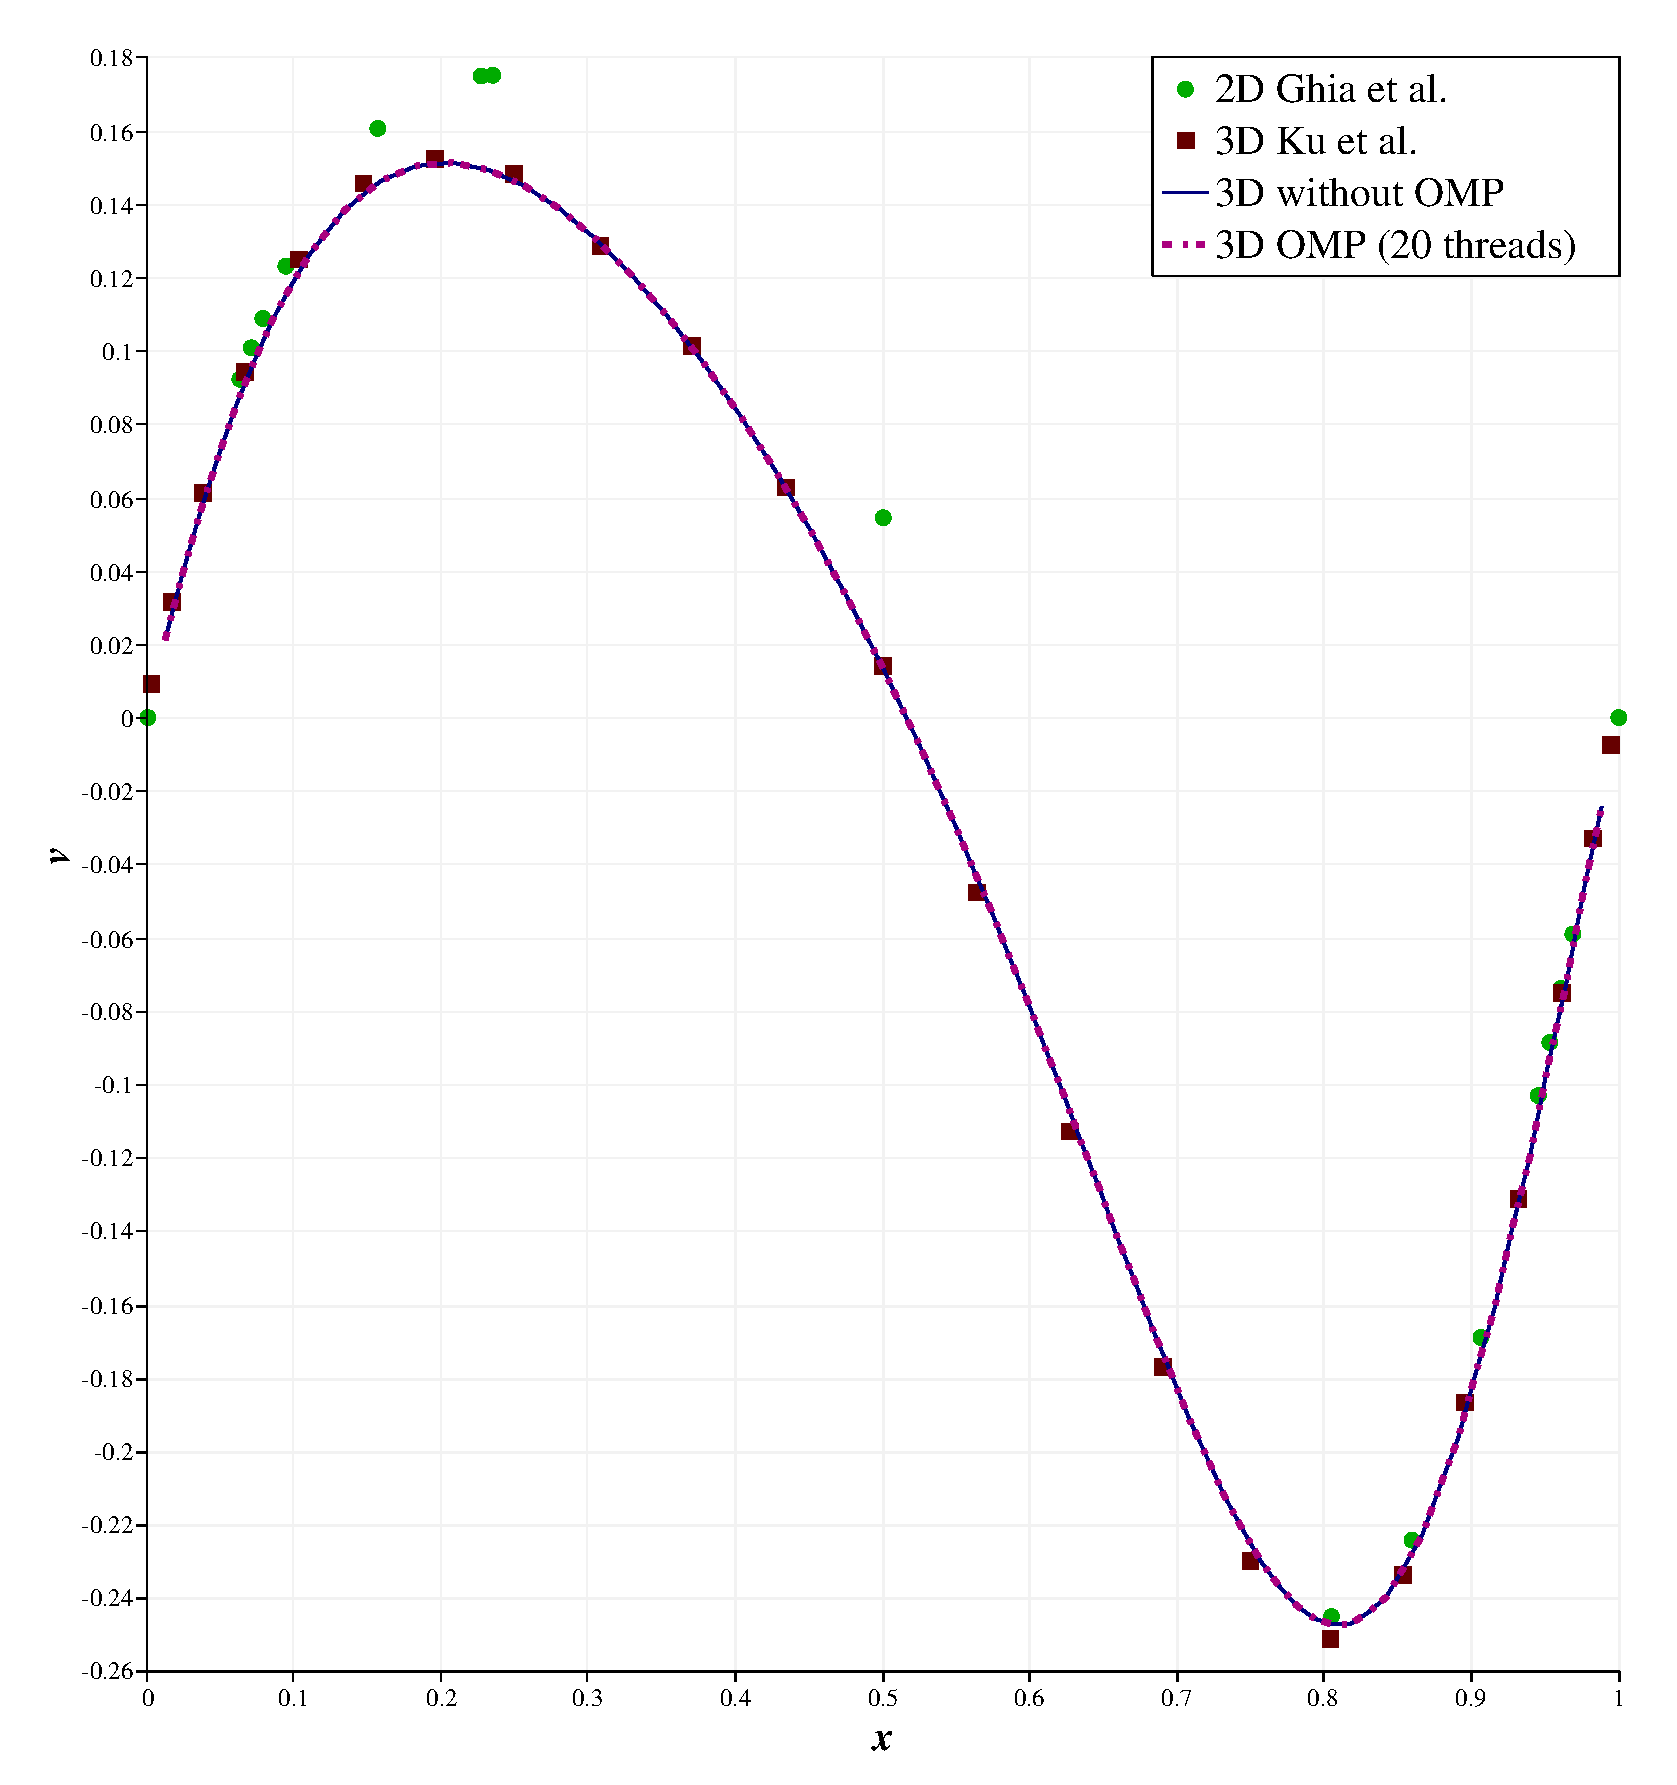
\includegraphics[width=\linewidth]{V-3D_ompValidation.eps}
    \caption{\(v\)-velocity profiles on the horizontal centerline in cubic cavity (at the center of \(z\)-axis) for the various cases.}
\end{figure}

The results of the parallelized code are also in very good agreement with the three-dimensional results of Ku et al \cite{Ku:1987:PMS:33136.33145} and match the non-parallelized version's results exactly. The differences with two-dimensional flow are apparent due to the effect of three-dimensional boundary conditions.

\begin{table}[H]
    \centering
    \begin{tabular}{@{}lll@{}}
        \toprule
        Number of threads & Simulation time & Reduction in time \\
        & (minutes) & (\%) \\
        \midrule
        1 (old code) & 376 & - \\
        1 (revised code) & 333 & - \\
        4 & 103 & 69.1 \\
        5 & 87 & 79.9 \\
        10 & 55 & 83.5 \\
        12 & 50 & 85.0 \\
        18 & 45 & 86.5 \\
        20 & 40 & 88.0 \\
        \bottomrule
    \end{tabular}
    \caption{Comparison of simulation times for different number of threads after parallelization with OpenMP, for a grid size of \(41\times41\times41(=68,921)\).}
\end{table}


% References
\bibliographystyle{unsrt}
\bibliography{33145.bib,0021999182900584.bib}

\end{document}
